\section[\textcolor{\statusSecFive}{[Expt] VGGT Omega Initialization}]{\textcolor{\statusSecFive}{[Expt] VGGT Omega Initialization}}

\begin{tcolorbox}[title={Status: [Full Pipeline Active / Exp 1 Deprecated]}, colframe=\statusSecFive, colback=\statusSecFive!5]
\textbf{Aim / Why:} To implement a modular add-on utilizing the \texttt{vggt\_omega} model to improve MeshSplatting:
\begin{itemize}
    \item \textbf{\textcolor{red}{Exp 1 (DEPRECATED):}} Attempting to align VGGT geometry with COLMAP cameras via PCA (\texttt{--vggt\_mode geometry\_only}) was found to be \textbf{utter nonsense}. Mixing coordinate frames creates rendering corruption and is strictly prohibited.
    \item \textbf{Exp 2 (Full Pipeline):} A pure, COLMAP-free pipeline that natively uses both the point cloud and camera poses directly from VGGT Omega (\texttt{--vggt\_mode full\_pipeline}).
\end{itemize}
\end{tcolorbox}

\subsection{Execution \& Technical Details}
\begin{itemize}
    \item \textbf{Implementation Strategy (Plug-and-Play)}: The feature is completely modular, controlled via the \texttt{--vggt\_mode} flag (\texttt{geometry\_only} for Exp 1, \texttt{full\_pipeline} for Exp 2). When empty, the pipeline runs the default COLMAP SfM initialization perfectly untouched.
    \item \textbf{Data Pipeline Integration}:
    \begin{itemize}
        \item A new \texttt{VGGTParams} argument group handles the configuration.
        \item Custom dataloader functions (\texttt{load\_vggt\_omega\_pcd} and \texttt{readVGGTSceneInfo}) are implemented in \texttt{scene/dataset\_readers.py}.
    \end{itemize}
    \item \textbf{Alignment Algorithm (PCA for Exp 1)}:
    \begin{itemize}
        \item To use VGGT geometry with COLMAP cameras (Exp 1), the VGGT points are shifted so their centroid matches COLMAP.
        \item An RMS (Root Mean Square) distance from the centroid is calculated, and VGGT points are scaled by $S_{colmap} / S_{vggt}$.
        \item Rotation is handled via Principal Component Analysis (PCA) to align the dominant axes of the geometries without point-to-point correspondences.
    \end{itemize}
    \item \textbf{Depth Map Alignment (Z-Buffer Projection for Exp 2)}:
    \begin{itemize}
        \item Since Exp 2 uses dense points without explicit 2D-3D keypoint mappings, \texttt{make\_depth\_scale\_vggt.py} uses a Z-buffer projection logic.
        \item VGGT points are projected into the VGGT cameras to generate a depth map, which is then used to align the raw monocular depth maps (\texttt{Depth Anything V2}) to the VGGT scale.
    \end{itemize}
\end{itemize}

\subsection{Visualization: Initialization Flow Comparison (High-Level)}
\begin{center}
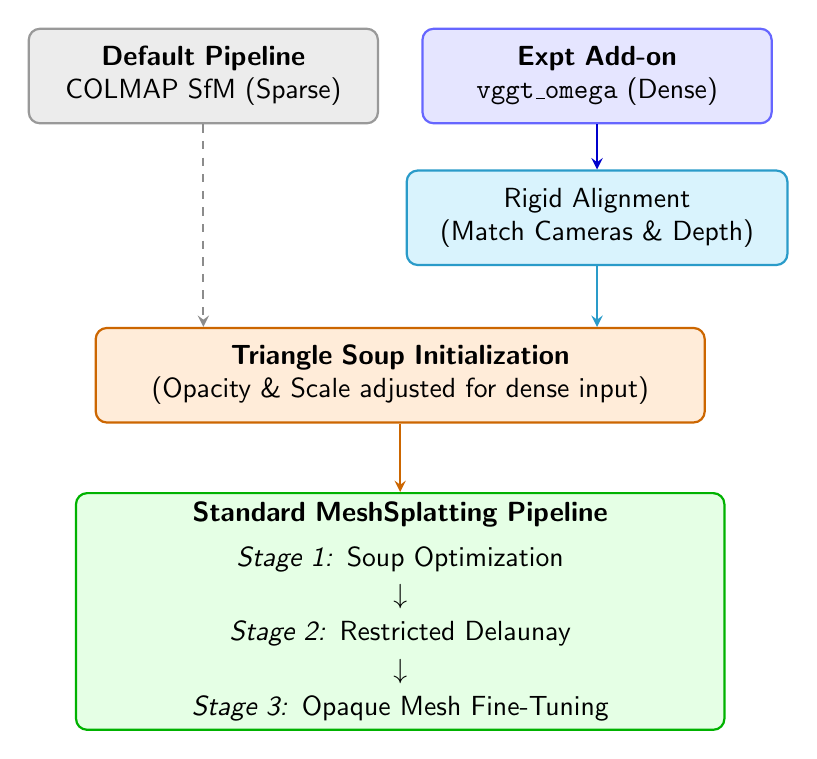
\begin{tikzpicture}[
  font=\sffamily,
  colmapbox/.style={rectangle, rounded corners=4pt, minimum height=1.2cm, text centered, text width=4.2cm, draw=gray!80, fill=gray!15, thick},
  vggtbox/.style={rectangle, rounded corners=4pt, minimum height=1.2cm, text centered, text width=4.2cm, draw=blue!60, fill=blue!10, thick},
  alignbox/.style={rectangle, rounded corners=4pt, minimum height=1.2cm, text centered, text width=4.6cm, draw=cyan!80!black, fill=cyan!15, thick},
  initbox/.style={rectangle, rounded corners=4pt, minimum height=1.2cm, text centered, text width=7.5cm, draw=orange!80!black, fill=orange!15, thick},
  pipelinebox/.style={rectangle, rounded corners=4pt, minimum height=2cm, text centered, text width=8cm, draw=green!70!black, fill=green!10, thick},
  arr/.style={thick, ->, >=stealth}
]

\node (colmap) [colmapbox] at (1.5, 0) {\textbf{Default Pipeline}\\COLMAP SfM (Sparse)};
\node (vggt) [vggtbox] at (6.5, 0) {\textbf{Expt Add-on}\\ \texttt{vggt\_omega} (Dense)};
\node (align) [alignbox] at (6.5, -1.8) {Rigid Alignment\\(Match Cameras \& Depth)};
\node (init) [initbox] at (4.0, -3.8) {\textbf{Triangle Soup Initialization}\\(Opacity \& Scale adjusted for dense input)};
\node (train) [pipelinebox] at (4.0, -6.8) {\textbf{Standard MeshSplatting Pipeline}\\[0.15cm] \textit{Stage 1:} Soup Optimization\\[0.05cm] $\downarrow$\\[0.05cm] \textit{Stage 2:} Restricted Delaunay\\[0.05cm] $\downarrow$\\[0.05cm] \textit{Stage 3:} Opaque Mesh Fine-Tuning};

\draw [arr, dashed, gray!90] (colmap.south) -- (colmap.south |- init.north);
\draw [arr, blue!80!black] (vggt.south) -- (align.north);
\draw [arr, cyan!80!black] (align.south) -- (align.south |- init.north);
\draw [arr, orange!80!black] (init.south) -- (train.north);

\end{tikzpicture}
\end{center}

\newpage
\subsection{Detailed Visualization: Experiment 1 (Geometry Ablation)}
\begin{center}
\resizebox{\textwidth}{!}{
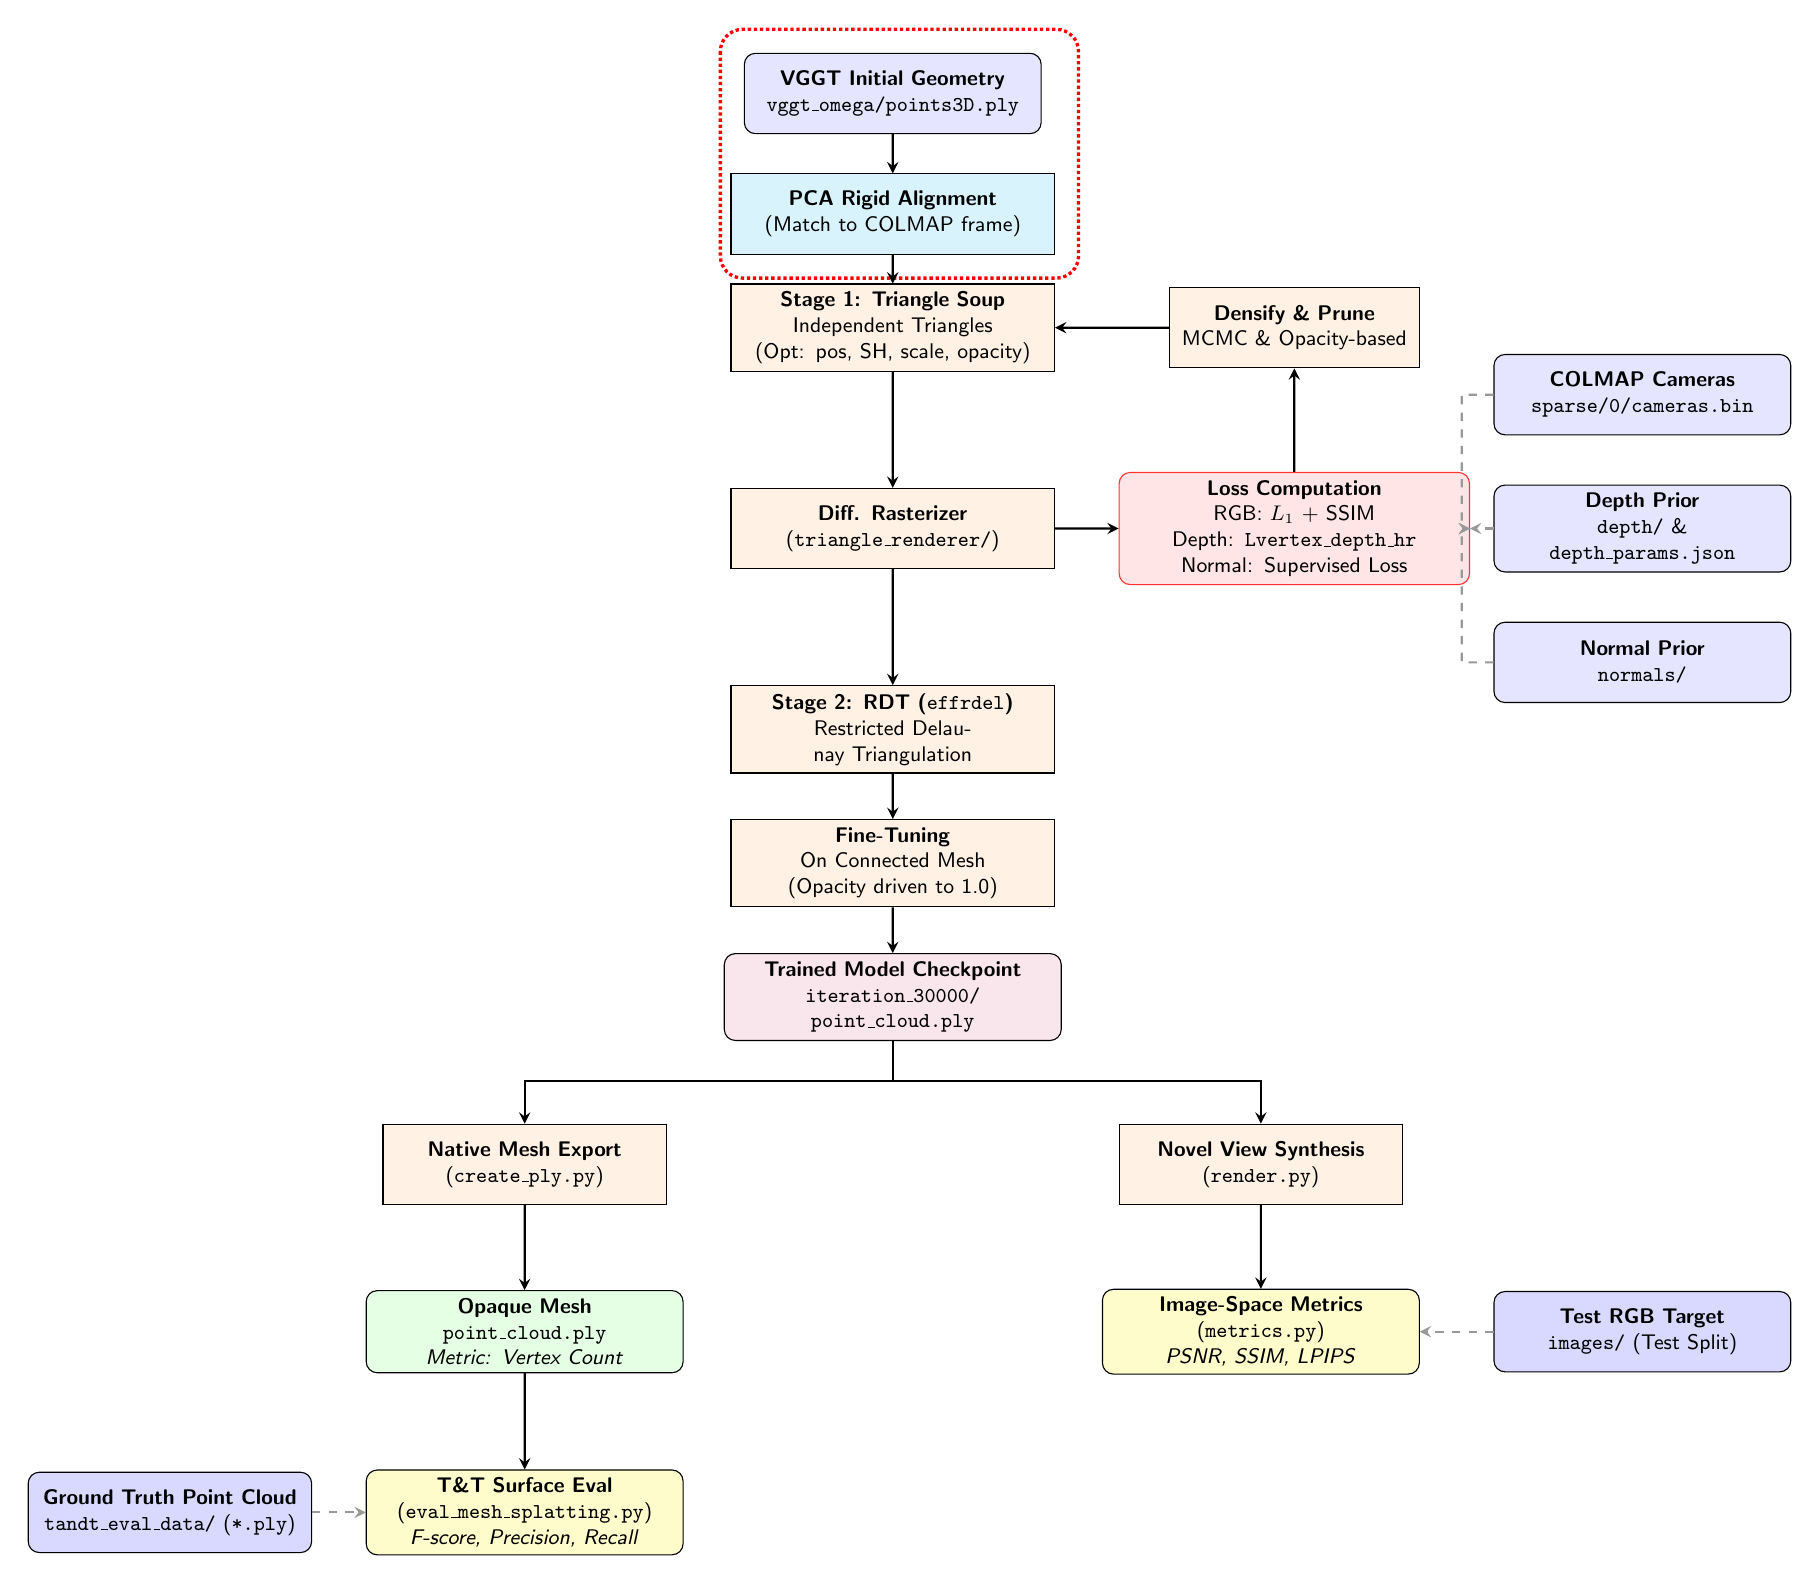
\begin{tikzpicture}[
    scale=0.85, transform shape,
    font=\sffamily\small,
    data/.style={rectangle, rounded corners, draw=black, fill=blue!10, text centered, minimum height=1.2cm, text width=4.2cm},
    process/.style={rectangle, draw=black, fill=orange!10, text centered, minimum height=1.2cm, text width=4.6cm},
    loss/.style={rectangle, rounded corners, draw=red!80, fill=red!10, text centered, minimum height=1.2cm, text width=5.0cm},
    output/.style={rectangle, rounded corners, draw=black, fill=green!10, text centered, minimum height=1.2cm, text width=4.8cm},
    arrow/.style={thick, ->, >=stealth},
    dashed_arrow/.style={thick, dashed, ->, >=stealth, draw=gray!80},
    changed/.style={draw=red, densely dotted, very thick, rounded corners=8pt}
]

% --- Nodes ---
% Center Column (Training)
\node (pts) at (0, 0) [data] {\textbf{VGGT Initial Geometry}\\ \texttt{vggt\_omega/points3D.ply}};
\node (align) at (0, -1.8) [process, fill=cyan!15] {\textbf{PCA Rigid Alignment}\\ (Match to COLMAP frame)};
\node (soup) at (0, -3.5) [process] {\textbf{Stage 1: Triangle Soup}\\ Independent Triangles\\ (Opt: pos, SH, scale, opacity)};
\node (render) at (0, -6.5) [process] {\textbf{Diff. Rasterizer}\\ (\texttt{triangle\_renderer/})};
\node (rdt) at (0, -9.5) [process] {\textbf{Stage 2: RDT (\texttt{effrdel})}\\ Restricted Delaunay Triangulation};
\node (finetune) at (0, -11.5) [process] {\textbf{Fine-Tuning}\\ On Connected Mesh\\ (Opacity driven to 1.0)};
\node (ckpt) at (0, -13.5) [data, fill=purple!10, text width=4.8cm] {\textbf{Trained Model Checkpoint}\\ \texttt{iteration\_30000/}\\\texttt{point\_cloud.ply}};

% Highlights for Exp 1 Changes
\draw [changed] ([xshift=-10pt,yshift=10pt]pts.north west) rectangle ([xshift=10pt,yshift=-10pt]align.south east);

% Right Column (Training Loop)
\node (densify) at (6, -3.5) [process, text width=3.5cm] {\textbf{Densify \& Prune}\\ MCMC \& Opacity-based};
\node (losses) at (6, -6.5) [loss] {\textbf{Loss Computation}\\ RGB: $L_1$ + SSIM\\ Depth: \texttt{Lvertex\_depth\_hr}\\ Normal: Supervised Loss};

% Far Right Column (Data Priors - Unchanged COLMAP ones)
\node (imgs) at (11.2, -4.5) [data] {\textbf{COLMAP Cameras}\\ \texttt{sparse/0/cameras.bin}};
\node (depth) at (11.2, -6.5) [data] {\textbf{Depth Prior}\\ \texttt{depth/} \&\\ \texttt{depth\_params.json}};
\node (norms) at (11.2, -8.5) [data] {\textbf{Normal Prior}\\ \texttt{normals/}};

% --- Evaluation Nodes (Bottom) ---
\node (create_ply) at (-5.5, -16) [process, text width=4cm] {\textbf{Native Mesh Export}\\ (\texttt{create\_ply.py})};
\node (render_py) at (5.5, -16) [process, text width=4cm] {\textbf{Novel View Synthesis}\\ (\texttt{render.py})};

\node (out_native) at (-5.5, -18.5) [output, text width=4.5cm] {\textbf{Opaque Mesh}\\ \texttt{point\_cloud.ply}\\ \textit{Metric: Vertex Count}};
\node (eval_metrics) at (5.5, -18.5) [output, fill=yellow!20, text width=4.5cm] {\textbf{Image-Space Metrics}\\ (\texttt{metrics.py})\\ \textit{PSNR, SSIM, LPIPS}};

% Test Data for Metrics
\node (test_imgs) at (11.2, -18.5) [data, fill=blue!15] {\textbf{Test RGB Target}\\ \texttt{images/} (Test Split)};
\node (eval_tandt) at (-5.5, -21.2) [output, fill=yellow!20, text width=4.5cm] {\textbf{T\&T Surface Eval}\\ (\texttt{eval\_mesh\_splatting.py})\\ \textit{F-score, Precision, Recall}};
\node (gt_data) at (-10.8, -21.2) [data, fill=blue!15, text width=4cm] {\textbf{Ground Truth Point Cloud}\\ \texttt{tandt\_eval\_data/} (\texttt{*.ply})};

% --- Edges ---
\draw [arrow] (pts) -- (align);
\draw [arrow] (align) -- (soup);
\draw [arrow] (soup) -- (render);
\draw [arrow] (render) -- (rdt);
\draw [arrow] (rdt) -- (finetune);
\draw [arrow] (finetune) -- (ckpt);

% Loop flow
\draw [arrow] (render) -- (losses);
\draw [arrow] (losses) -- (densify);
\draw [arrow] (densify) -- (soup);

% Data Priors flowing into Losses
\draw [dashed_arrow] (imgs.west) -- (8.5, -4.5) |- (losses.east);
\draw [dashed_arrow] (depth.west) -- (losses.east);
\draw [dashed_arrow] (norms.west) -- (8.5, -8.5) |- (losses.east);

% Branching to Evaluation
\draw [arrow] (ckpt.south) -- +(0, -0.6) -| (create_ply.north);
\draw [arrow] (ckpt.south) -- +(0, -0.6) -| (render_py.north);

% Evaluation pipelines
\draw [arrow] (create_ply) -- (out_native);
\draw [arrow] (render_py) -- (eval_metrics);
\draw [dashed_arrow] (test_imgs.west) -- (eval_metrics.east);
\draw [arrow] (out_native) -- (eval_tandt);
\draw [dashed_arrow] (gt_data.east) -- (eval_tandt.west);

\end{tikzpicture}
}
\end{center}

\newpage
\subsection{Detailed Visualization: Experiment 2 (COLMAP-Free Pipeline)}
\begin{center}
\resizebox{\textwidth}{!}{
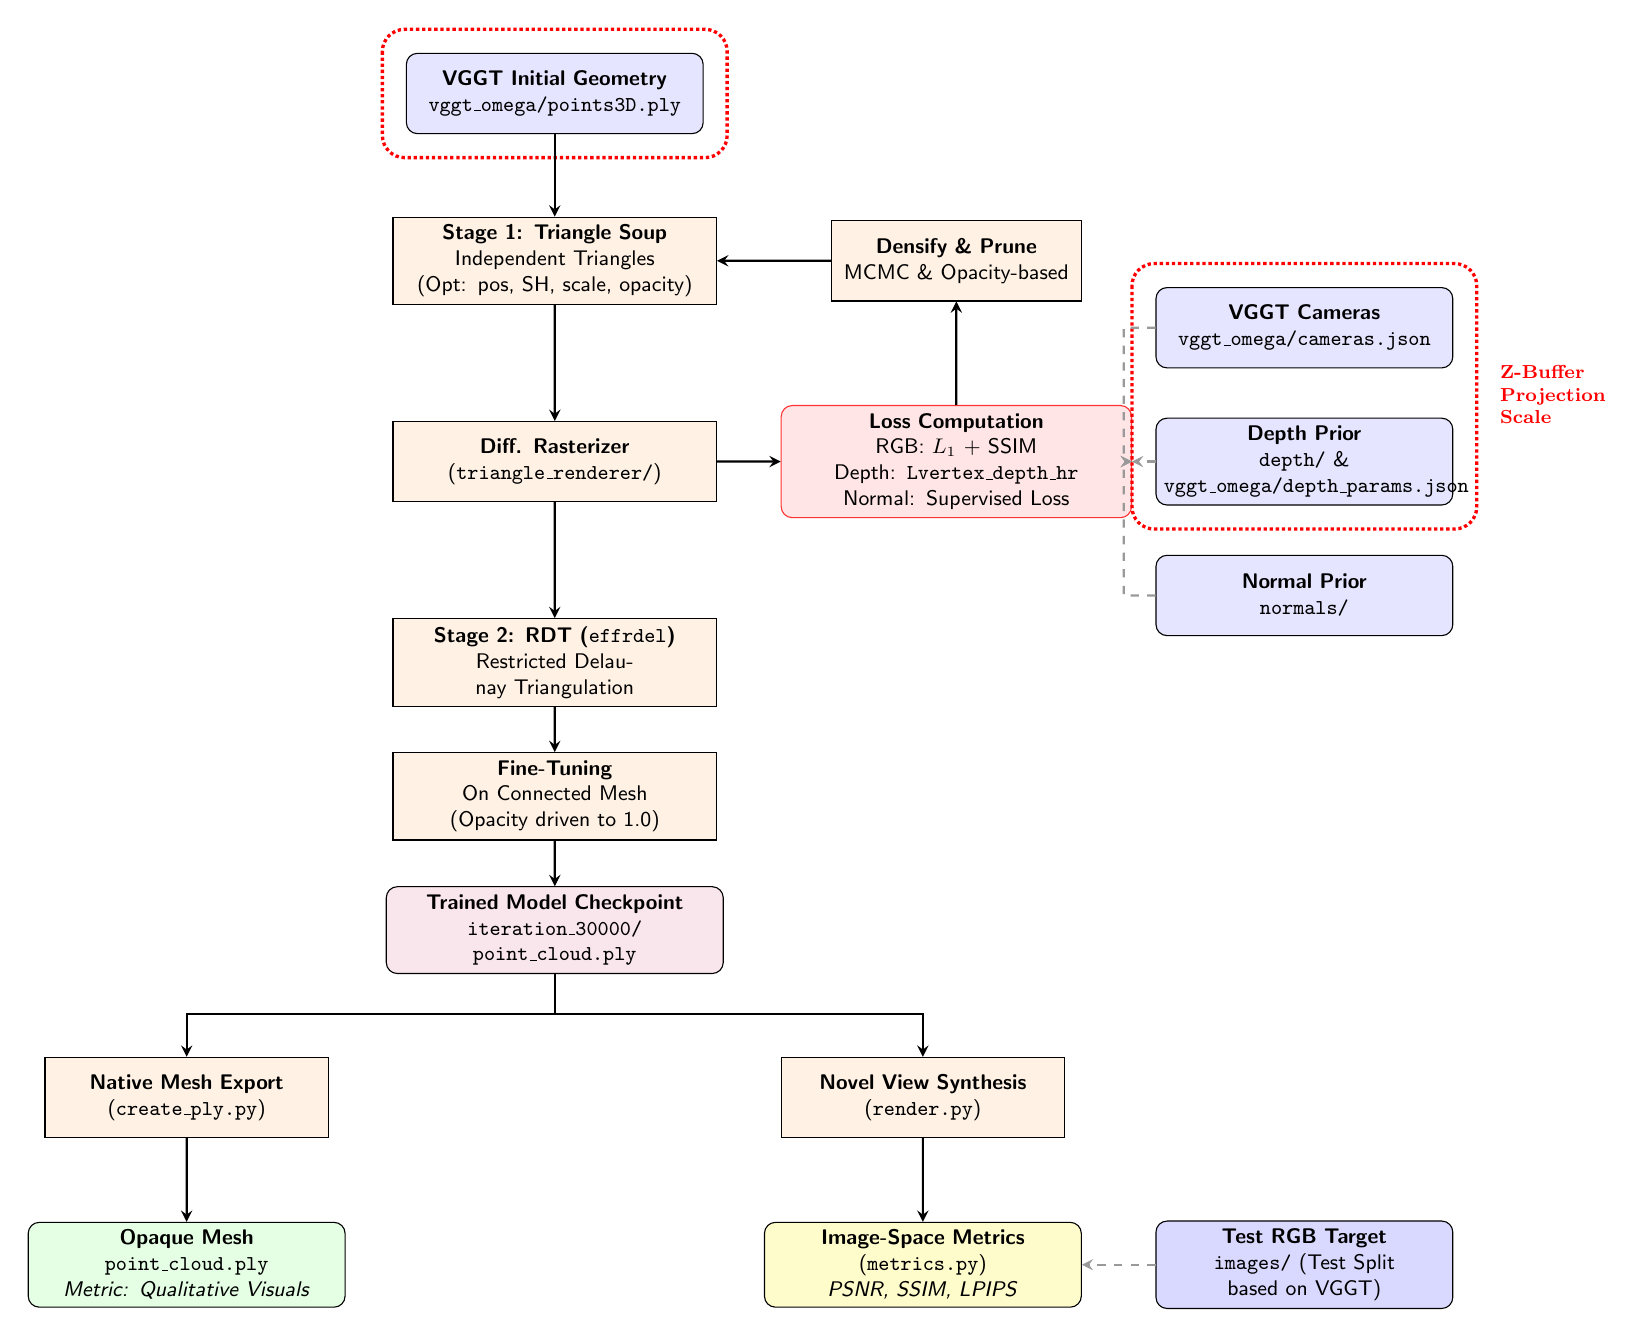
\begin{tikzpicture}[
    scale=0.85, transform shape,
    font=\sffamily\small,
    data/.style={rectangle, rounded corners, draw=black, fill=blue!10, text centered, minimum height=1.2cm, text width=4.2cm},
    process/.style={rectangle, draw=black, fill=orange!10, text centered, minimum height=1.2cm, text width=4.6cm},
    loss/.style={rectangle, rounded corners, draw=red!80, fill=red!10, text centered, minimum height=1.2cm, text width=5.0cm},
    output/.style={rectangle, rounded corners, draw=black, fill=green!10, text centered, minimum height=1.2cm, text width=4.8cm},
    arrow/.style={thick, ->, >=stealth},
    dashed_arrow/.style={thick, dashed, ->, >=stealth, draw=gray!80},
    changed/.style={draw=red, densely dotted, very thick, rounded corners=8pt}
]

% --- Nodes ---
% Center Column (Training)
\node (pts) at (0, 0) [data] {\textbf{VGGT Initial Geometry}\\ \texttt{vggt\_omega/points3D.ply}};
\node (soup) at (0, -2.5) [process] {\textbf{Stage 1: Triangle Soup}\\ Independent Triangles\\ (Opt: pos, SH, scale, opacity)};
\node (render) at (0, -5.5) [process] {\textbf{Diff. Rasterizer}\\ (\texttt{triangle\_renderer/})};
\node (rdt) at (0, -8.5) [process] {\textbf{Stage 2: RDT (\texttt{effrdel})}\\ Restricted Delaunay Triangulation};
\node (finetune) at (0, -10.5) [process] {\textbf{Fine-Tuning}\\ On Connected Mesh\\ (Opacity driven to 1.0)};
\node (ckpt) at (0, -12.5) [data, fill=purple!10, text width=4.8cm] {\textbf{Trained Model Checkpoint}\\ \texttt{iteration\_30000/}\\\texttt{point\_cloud.ply}};

% Right Column (Training Loop)
\node (densify) at (6, -2.5) [process, text width=3.5cm] {\textbf{Densify \& Prune}\\ MCMC \& Opacity-based};
\node (losses) at (6, -5.5) [loss] {\textbf{Loss Computation}\\ RGB: $L_1$ + SSIM\\ Depth: \texttt{Lvertex\_depth\_hr}\\ Normal: Supervised Loss};

% Far Right Column (Data Priors)
\node (imgs) at (11.2, -3.5) [data] {\textbf{VGGT Cameras}\\ \texttt{vggt\_omega/cameras.json}};
\node (depth) at (11.2, -5.5) [data] {\textbf{Depth Prior}\\ \texttt{depth/} \&\\ \texttt{vggt\_omega/depth\_params.json}};
\node (norms) at (11.2, -7.5) [data] {\textbf{Normal Prior}\\ \texttt{normals/}};

% Highlights for Exp 2 Changes
\draw [changed] ([xshift=-10pt,yshift=10pt]pts.north west) rectangle ([xshift=10pt,yshift=-10pt]pts.south east);
\draw [changed] ([xshift=-10pt,yshift=10pt]imgs.north west) rectangle ([xshift=10pt,yshift=-10pt]depth.south east);
\node[text=red, font=\footnotesize, align=left, anchor=west] at (14.0, -4.5) {\textbf{Z-Buffer}\\ \textbf{Projection}\\ \textbf{Scale}};

% --- Evaluation Nodes (Bottom) ---
\node (create_ply) at (-5.5, -15) [process, text width=4cm] {\textbf{Native Mesh Export}\\ (\texttt{create\_ply.py})};
\node (render_py) at (5.5, -15) [process, text width=4cm] {\textbf{Novel View Synthesis}\\ (\texttt{render.py})};

\node (out_native) at (-5.5, -17.5) [output, text width=4.5cm] {\textbf{Opaque Mesh}\\ \texttt{point\_cloud.ply}\\ \textit{Metric: Qualitative Visuals}};
\node (eval_metrics) at (5.5, -17.5) [output, fill=yellow!20, text width=4.5cm] {\textbf{Image-Space Metrics}\\ (\texttt{metrics.py})\\ \textit{PSNR, SSIM, LPIPS}};

% Test Data for Metrics
\node (test_imgs) at (11.2, -17.5) [data, fill=blue!15] {\textbf{Test RGB Target}\\ \texttt{images/} (Test Split based on VGGT)};

% --- Edges ---
\draw [arrow] (pts) -- (soup);
\draw [arrow] (soup) -- (render);
\draw [arrow] (render) -- (rdt);
\draw [arrow] (rdt) -- (finetune);
\draw [arrow] (finetune) -- (ckpt);

% Loop flow
\draw [arrow] (render) -- (losses);
\draw [arrow] (losses) -- (densify);
\draw [arrow] (densify) -- (soup);

% Data Priors flowing into Losses
\draw [dashed_arrow] (imgs.west) -- (8.5, -3.5) |- (losses.east);
\draw [dashed_arrow] (depth.west) -- (losses.east);
\draw [dashed_arrow] (norms.west) -- (8.5, -7.5) |- (losses.east);

% Branching to Evaluation
\draw [arrow] (ckpt.south) -- +(0, -0.6) -| (create_ply.north);
\draw [arrow] (ckpt.south) -- +(0, -0.6) -| (render_py.north);

% Evaluation pipelines
\draw [arrow] (create_ply) -- (out_native);
\draw [arrow] (render_py) -- (eval_metrics);
\draw [dashed_arrow] (test_imgs.west) -- (eval_metrics.east);

\end{tikzpicture}
}
\end{center}
